\section{Problem 3-1 Clustering Coefficients}

\begin{enumerate}
	\item Given an undirected complete graph with $N$ nodes, calculate the total number of triangles. Note that the order of nodes matters, e.g., $A \rightarrow B \rightarrow C$ is not the same as $C \rightarrow B \rightarrow A$.
	
	First one needs to find the number of unique triangles in the complete graph, which is calculated by $\binom{N}{3}$. For the calculation of the global clustering coefficient, this is the amount of triangles to be used and matches the post on Moodle from Shideh Almasian:
	
	\begin{quote}
		\textit{I delete the post and the comments because my answer was wrong. So the correct answer is that "the order of nodes does **not** matter", ABC is a single triangle and that counts towards the global clustering coefficient.}
	\end{quote}

	In case one additionally wants to define the total number of triangles by the order of nodes, one has multiply with $3!$. So the total number of triangles in a complete graph asked by the task description is $3! \cdot \binom{N}{3}$.
	
	\item Can the number of triangles in a graph be larger than the number of edges? Are you able to find a graph with more triangles than edges? If so, draw such a graph.
	
	We use the stricter definition of the number of triangles in a graph that does not consider the order of nodes. We again use the example of a complete graph. The number of edges in such a graph is defined by $L=\binom{N}{2}=\frac{N(N-1)}{2}$. $\binom{N}{3} > \binom{N}{2}$ holds for $N=6$. See the following graph in Figure \ref{clique}:
	
	\begin{figure}[h]
		\centering
		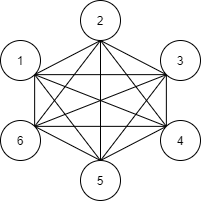
\includegraphics[width=0.25\linewidth]{images/clique.png}
		\caption{A complete graph with $N=6$.}
		\label{clique}
	\end{figure}

	This means the number of triangles in a graph can be larger than the number of edges.
	
	\item Prove that the number of connected triples in an undirected graph is equal to half the \textbf{sum} of non-zero off-diagonal entries of the adjacency matrix $A^2$, where $A$ denotes the adjacency matrix.
	
	Let $(n_i, n_j, n_k)$ be a connected triple in a graph with $N \ge 3$. This means that there is a path from $n_i$ to $n_k$ of length 2. We know that for such a path is must hold $A_{ij}A_{jk} = 1$. Therefore, $A^2$ holds paths of length 2, i.e. connected triples in its non-zero off-diagonal entries. As an illustration, consider the following simple graph in Figure \ref{triples} and the following Equation \ref{equation}:
	
	\begin{figure}[h]
		\centering
		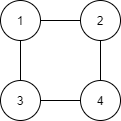
\includegraphics[width=0.25\linewidth]{images/triples.png}
		\caption{A simple graph with 4 connected triples.}
		\label{triples}
	\end{figure}
	
	\begin{equation*} \label{equation}
		\begin{pmatrix}
			0 & 1 & 1 & 0\\
			1 & 0 & 0 & 1\\
			1 & 0 & 0 & 1\\
			0 & 1 & 1 & 0
		\end{pmatrix}
		\begin{pmatrix}
			0 & 1 & 1 & 0\\
			1 & 0 & 0 & 1\\
			1 & 0 & 0 & 1\\
			0 & 1 & 1 & 0
		\end{pmatrix} = 
		\begin{pmatrix}
			2 & 0 & 0 & 2\\
			0 & 2 & 2 & 0\\
			0 & 2 & 2 & 0\\
			2 & 0 & 0 & 2
		\end{pmatrix}
	\end{equation*}

	Half the sum of all non-zero off-diagonal entries of the adjacency matrix $A^2$ equals exactly the number of connected triples, namely 4. 
	
	\item Given a graph with its adjacency matrix $A$, find an expression for the global clustering coefficient in terms of the elements of the adjacency matrix. Notice that the number of triangles in a graph is \textbf{related} to the trace of the matrix $A^3$.
	
	We know 
	
	\begin{equation*}
		C = \frac{3 \cdot \#triangles}{\#connected \; triples}.
	\end{equation*}
	
	The also know that the relation between the number of triangles $n_{triangles}$ and the trace of $A^3$ is exactly $6 \cdot n_{triangles} = tr(A^3)$. Therefore it follows:
	
	\begin{equation*}
		C = \frac{tr(A^3)}{\sum_{i \neq j} A^2_{ij}}
	\end{equation*}

\end{enumerate}